\documentclass[12pt,letterpaper]{article}

\pdfoutput=1

\usepackage[OT1]{fontenc}
\usepackage[colorlinks,citecolor=blue,urlcolor=blue]{hyperref}
\usepackage[pdftex]{graphicx}
\usepackage{subfig}
\usepackage{fullpage}
\usepackage{palatino}
\usepackage{mathpazo}
\usepackage{amsmath}
\usepackage{amssymb}
\usepackage{color}
\usepackage{todonotes}
\usepackage{listings}
\usepackage{framed}
\usepackage{common}
\usepackage{graphicx}
\graphicspath{ {sec7_dendrogram/} }
\usepackage[mmddyyyy,hhmmss]{datetime}


\newboolean{solutionCopy}
\setboolean{solutionCopy}{false} 

\ifthenelse{\boolean{solutionCopy}}{
  \includeversion{solution}
}{
  \excludeversion{solution}
}


\begin{document}

\ifthenelse{\boolean{solutionCopy}}{
\begin{center}
{\LARGE CS 181 Spring 2018 Section 7\\
Clustering\\
Solution}
\end{center}
}{
  \begin{center}
{\LARGE CS 181 Spring 2018 Section 7}\\
Clustering
\end{center}
}




\section{Motivation}
We now move onto \textbf{unsupervised learning}, where the objective is to learn the structure of unlabeled data. In other words, we are looking for groups, or \textbf{clusters} among the data. Clustering algorithms are useful not only for finding groups in data, but also to extract features of the data that summarize the most important information about the data in a compressed way. \\
For most clustering algorithms, we need some kind of a metric that we can use to specify the notion of "distance" between the data points. If, for example, the points $\textbf{x}$ and $\textbf{x'}$ live in some Euclidean space $\mathbb{R}^m$, then the natural choice of such metric is the $l_2$ distance:
\begin{align*}
	 ||\textbf{x} - \textbf{x'}|| &= \sqrt{\sum_{i = 1}^{n}(x_i - x_i')^2}
\end{align*}

Now that the metric is well-defined, the next thing we need to do is to decide how many groups we want. Sometimes you know the ideal number of groups in advance (\textit{e.g.} clustering alphabet). Other times, you need to decide if you'd like a more compressed representation with more information loss by having the number of groups small, or a less compressed representation with less information loss by having the number of groups large. \\
Suppose our data set is $\{\textbf{x}_i\}_{i=1}^{n}$, then our objective is to find the ideal assignment of the data set to the clusters, by assigning to each of the $n$ data points, a binary \textbf{responsibility vector} $\textbf{r}_i$, which is all zeros except one component, which corresponds to the assigned cluster.

\section{K-Means Algorithm}
The idea is to represent each cluster by the point in data space that is the average of the data assigned to it. For some choice of $K$, 
the K-Means Algorithm (also called Lloyd's algorithm)
keeps doing the following: iterate through the data points and update the responsibility vectors according to their closest means,
and iterate over the mean vectors $\{\bmu_k\}_{k=1}^{K}$ 
and change them to be the mean of the examples currently assigned the cluster. 
%After that, we
%
We repeat this until convergence: until none of the responsibility vectors change.
% \\
%(\textit{The pseudocode for Lloyd's Algorithm should be reviewed in section.})

\subsection{Derivation}
We begin by defining a loss function:
\begin{align*}
	 \mcL(\{\textbf{r}_i\}_{i=1}^n,\{\bmu_k\}_{k=1}^K) &= \sum_{i=1}^{n}\sum_{k=1}^{K} r_{ik} ||\textbf{x}_i - \bmu_k ||^2
\end{align*}
and the K-Means Algorithm minimizes this via coordinate descent.
We first choose $r_{i}$ such that:
\begin{align*}
	 r_{ik} &= \begin{cases}
	 	1 & \mbox{if }k = argmin_{k'}||\textbf{x}_i - \bmu_{k'}|| \\
	 	0 & \mbox{otherwise}
	 \end{cases}
\end{align*}

Having fixed everything else, we see that it is equivalent, for a given
$k$, to minimize the square loss:
%
\begin{align*}
	 \mcL(\bmu_k) &= \sum_{i=1}^{n} r_{ik} ||\textbf{x}_i -\bmu_k||^2 \\
	 &= \sum_{i=1}^{n} r_{ik} (\textbf{x}_i - \bmu_k)^T(\textbf{x}_i - \bmu_k)
\end{align*}
Taking the derivative and setting it to zero,
\begin{align*}
	 \frac{\partial \mcL(\bmu_k)}{\partial \bmu_k} &= -2 \sum_{i = 1}^{n} r_{ik} (\textbf{x}_i - \bmu_k) = 0 \\
	 \bmu_k &= \frac{\sum_{i=1}^n r_{ik}\textbf{x}_i}{\sum_{i=1}^{n}r_{ik}}
\end{align*}

\subsection{Number of Clusters}

\if 0
Our main approach is to use the idea of the \textbf{gap statistic}. We can define the within-cluster dispersion:
\begin{align*}
	 D_k &= \sum_{i=1}^{n} \sum_{i'=1}^{n} r_{ik} r_{i'k} ||\textbf{x}_i - \textbf{x'}_i||^2
\end{align*}
Then the dispersion for the clustering is the normalized sum of the within-cluster dispersion over all the clusters:
\begin{align*}
	 W_k &= \sum_{k=1}^{K} \frac{1}{2\sum_{i=1}^{n} r_{ik}} \sum_{i=1}^{n} \sum_{i'=1}^{n} r_{ik} r_{i'k} ||\textbf{x}_i - \textbf{x'}_i||^2
\end{align*}
To compute the gap statistic, we use a null distribution for the data, from which we generate reference data. Then, the gap statistic can be computed:
\begin{align*}
	 Gap_i(K) &= \mathbb{E}_{iull}[\log{W_K}] - \log{W_K} 
\end{align*}
\fi

There is not an especially well justified method to choose the number
of clusters when using K-means. One approach is to plot $K$ vs the
objective criterion, and look for a ``knee'' or ``kink'' where
progress slows down.

An advanced method is to use the ``gap statistic''. But this is out of
scope for the course.

\subsection{Notes}

Lloyd's algorithm finds a local optimal solution.  Finding the global
optimal is NP-hard. A common strategy is to use random restarts. More
recently, an algorithm called \textbf{K-Means++} has enjoyed popular
usage as an alternative to random initialization. This is out of scope
for the course, but the basic idea is to randomly select some of the
data to be the first cluster centers.  This is done by iteratively
adding cluster centers, sampling them in proportion to the squared
distance of each example from its nearest cluster center.  Thus
K-Means++ tends to favor points that are distant from the existing
centers and produce a more diverse set of centers.

It is generally a good idea to \textbf{standardize} the data to account for unsatisfying result due to dimension mismatch.
Lastly, when for the metric we are using for the given data set, a "mean" does not make sense, we might instead use a \textbf{K-Medoids Algorithm}. This algorithm requires the cluster centers to be a data point in the data set. 

\section{Hierarchical Agglomerative Clustering}

Hierarchical clustering constructs a tree over the data, where the leaves are individual data items, while the root is a single cluster that contains all of the data. When drawing the dendrogram, for the clustering to be valid, the distances between the two groups being merged should be monotonically increasing. 
%(\textit{The pseudocode for HAC should be reviewed in section.}) \\
The main decision in using
HAC is what the distance criterion should be between groups.

\subsection{The Min-Linkage Criterion}
For two groups indexed by $i$ and $i'$, the idea is to merge groups based on the shortest distance over all possible pairs:
\begin{align*}
	 \mathit{DIST}_{\mathrm{min}}(\{\boldx_i\}_{i=1}^{n}, \{\boldx_{i'}\}_{i'=1}^{n'}) &= \min_{i,i'}||\boldx_i - \boldx_{i'}||.
\end{align*}
%this produces the minimum spanning tree for the data.

\subsection{The Max-Linkage Criterion}
For two groups indexed by $i$ and $i'$, the idea is to merge groups based on the largest distance over all possible pairs:
\begin{align*}
	 \mathit{DIST}_{\mathrm{max}}(\{\boldx_i\}_{i=1}^{n}, \{\boldx_{i'}\}_{i'=1}^{n'})
 &= \max_{i,i'}||\boldx_i - \boldx_{i'}||
\end{align*}

\subsection{The Average-Linkage Criterion}
For two groups indexed by $i$ and $i'$, the idea is to average over all possible pairs between the groups:
\begin{align*}
	 \mathit{DIST}_{\mathrm{avg}}(\{\boldx_i\}_{i=1}^{n}, \{\boldx_{i'}\}_{i'=1}^{n'})
&= \frac{1}{nn'} \sum_{i=1}^{n} \sum_{i'=1}^{n'} ||\boldx_i - \boldx_{i'}||
\end{align*}

\subsection{The Centroid-Linkage Criterion}
For two groups indexed by $i$ and $i'$, the idea is to look at the difference between the groups' centroids:
\begin{align*}
	 \mathit{DIST}_{\mathrm{cent}}(\{\boldx_i\}_{i=1}^{n}, \{\boldx_{i'}\}_{i'=1}^{n'})
&= ||\left( \frac{1}{n} \sum_{i=1}^{n} \boldx_i \right) - \left( \frac{1}{n'} \sum_{i'=1}^{n'} \boldx_{i'} \right)||
\end{align*}

%\subsection{Divisive Clustering}
%While HAC is a bottom-up procedure, divising clustering is a top-down procedure, starting with a single group with all the data in it and then dividing and subdividing it into smaller groups using other clustering algorithms like K-Means or K-Medoids.
\newpage
\section{Practice Problems}
\begin{enumerate}

\item {\bf K-Means (Di Cook)}\\
\fbox{\parbox{\linewidth}{%
{Use K-means to cluster these examples in $\reals^2$, looking for $K = 2$ clusters. Suppose that points A and C are randomly selected as the initial means.
\\
\begin{center}
 \begin{tikzpicture}[x=1cm,y=.6cm]

\draw [dotted, gray] (-4,-4) grid (5,5);
 \draw[latex-latex, thin, draw=gray] (-4,0)--(4,0) node [right] {$x_1$}; % l'axe des abscisses
 \draw[latex-latex, thin, draw=gray] (0,-5)--(0,5) node [above] {$x_2$}; % l'axe des ordonnées
%  \draw[thick] (-3,-2)--(3,4); % l'axe des abscisses

\foreach \Point in {(1,1),(1,0), (0,2),(2,4),(3,5)}{
    \node at \Point {\textbullet};
}

% to ensure that the points are being properly centered:

\node [label={[shift={(.5,-1)}]B}] at (1,0) {$\circ$};
\node [label={[shift={(.5,-1)}]C}] at (0,2) {$\circ$};
\node [label={[shift={(.5,-1)}]D}] at (2,4) {$\circ$};
\node [label={[shift={(.5,-1)}]A}] at (1,1) {$\circ$};
\node [label={[shift={(.5,-1)}]E}] at (3,5) {$\circ$};

\end{tikzpicture}

\begin{tabular}{ |c|c|c| } 
 \hline
 Point & $x_1$ & $x_2$ \\ 
 \hline 
 A & 1 & 1 \\ 
 B & 1 & 0 \\ 
 C & 0 & 2 \\ 
 D & 2 & 4 \\
 E & 3 & 5 \\  
 \hline
\end{tabular}
\end{center}
}
}}
\begin{solution}
If we start with points A and C as our cluster, then let us set our cluster 1 mean $\bmu_1 = (1,1)$ and cluster 2 mean to be $\bmu_2 = (0,2)$. For each point, we will now calculate its distance from each cluster mean and assign it to the cluster where this distance is minimized.

For $\bmu = [1,1]$, $\bmu_2 = [0,2]$
\begin{center}
\begin{tabular}{ |c|c|c|c| } 
 \hline
 Point & $distc_1$ & $distc_2$  & $cluster$ \\ 
 \hline 
 A & 0 & $\sqrt{2}$ & 1 \\ 
 B & 1 & $\sqrt{5}$ & 1\\ 
 C & $\sqrt{2}$ & 0 & 2 \\ 
 D & $\sqrt{10}$ & $\sqrt{8}$ & 2\\
 E & $\sqrt{20}$ & $\sqrt{18}$ & 2\\  
 \hline
\end{tabular}
\end{center}
Now we want to update our cluster means so that it takes the average of the coordinates for all points assigned to this cluster. 
\begin{align*}
	\bmu_1= \frac{\sum_{i=1}^n r_{i1}\textbf{x}_i}{\sum_{i=1}^{n}r_{i1}} = [1, .5]\\
	\bmu_2= \frac{\sum_{i=1}^n r_{i2}\textbf{x}_i}{\sum_{i=1}^{n}r_{i2}} = [\frac{5}{3},\frac{11}{3}]\\
\end{align*}
\\
For $\bmu_1 = [1,.5]$, $\bmu_2 = [\frac{5}{3},\frac{11}{3}]$
\begin{center}
\begin{tabular}{ |c|c|c|c| } 
 \hline
 Point & $distc_1$ & $distc_2$  & $cluster$ \\ 
 \hline 
 A & .5 & $\sqrt{\frac{2}{3}^2 + \frac{8}{3}^2} = 2.7$ & 1\\ 
 B & .5  & $\sqrt{\frac{2}{3}^2 + \frac{11}{3}^2} = 3.7$ & 1\\ 
 C & $\sqrt{1+1.5^2} = 1.8$ & $\sqrt{\frac{5}{3}^2 + \frac{5}{3}^2} = 2.3$ & 1 \\ 
 D & $\sqrt{1+3.5^2} = 3.64$ & $\sqrt{\frac{1}{3}^2 + \frac{1}{3}^2} = .4$ & 2\\
 E & $\sqrt{2^2+4.5^2} = 4.9$ & $\sqrt{\frac{4}{3}^2 + \frac{4}{3}^2} = 1.9$ & 2\\  
 \hline
\end{tabular}
\end{center}
We will once again, recalculate our center means and distances from each point to the mean.
\begin{align*}
	\bmu_1= \frac{\sum_{i=1}^n r_{i1}\textbf{x}_i}{\sum_{i=1}^{n}r_{i1}} = [\frac{2}{3}, 1]\\
	\bmu_2= \frac{\sum_{i=1}^n r_{i2}\textbf{x}_i}{\sum_{i=1}^{n}r_{i2}} = [\frac{5}{2},\frac{9}{2}]\\
\end{align*}
For $\bmu_1 = [\frac{2}{3},1]$, $\bmu_2 = [\frac{5}{2},\frac{9}{2}]$
\begin{center}
\begin{tabular}{ |c|c|c|c| } 
 \hline
 Point & $distc_1 $& $distc_2$ & cluster \\ 
 \hline 
 A & $\sqrt{\frac{1}{3}^2} = .33$ & $\sqrt{\frac{3}{2}^2 + \frac{7}{2}^2} = 3.8$ & 1\\ 
 B &   $\sqrt{\frac{2}{3}^2 + 1} = 1.24$ &  $\sqrt{\frac{3}{2}^2 + \frac{9}{2}^2} = 4.7$ & 1\\ 
 C &  $\sqrt{\frac{2}{3}^2 + 1} = 1.24$& $\sqrt{\frac{5}{2}^2 + \frac{5}{2}^2} = 3.5$ & 1 \\ 
 D & $\sqrt{\frac{2}{3}^2 + 3^2} = 3.07$ & $\sqrt{\frac{1}{2}^2 + \frac{1}{2}^2} = .7$ & 2\\
 E & $\sqrt{\frac{7}{3}^2 + 4^2} = 4.63$ & $\sqrt{\frac{1}{2}^2 + \frac{1}{2}^2} = .7$& 2\\  
 \hline
\end{tabular}
\end{center}

We see that the $r_{ik}$ assignments have not changed, and therefore the means of the clusters do not change and the algorithm has converged. The final cluster assignments are shown below.

\begin{center}
 \begin{tikzpicture}[x=1cm,y=.6cm]

\draw [dotted, gray] (-4,-4) grid (5,5);
 \draw[latex-latex, thin, draw=gray] (-4,0)--(4,0) node [right] {$x_1$}; % l'axe des abscisses
 \draw[latex-latex, thin, draw=gray] (0,-5)--(0,5) node [above] {$x_2$}; % l'axe des ordonnées
%  \draw[thick] (-3,-2)--(3,4); % l'axe des abscisses

\foreach \Point in {(1,1),(1,0),(0,2)}{
    \node[color=red] at \Point {\textbullet};
}
\foreach \Point in {(2,4),(3,5)}{
    \node at \Point {\textbullet};
}

% to ensure that the points are being properly centered:

\node [label={[shift={(.5,-1)}]B}] at (1,0) {$\circ$};
\node [label={[shift={(.5,-1)}]C}] at (0,2) {$\circ$};
\node [label={[shift={(.5,-1)}]D}] at (2,4) {$\circ$};
\node [label={[shift={(.5,-1)}]A}] at (1,1) {$\circ$};
\node [label={[shift={(.5,-1)}]E}] at (3,5) {$\circ$};

\end{tikzpicture}
\end{center}
\end{solution}


\newpage

\item {\bf Convergence of K-Means (Bishop 9.1)}\\
\fbox{\parbox{\linewidth}{%
Consider Lloyd's algorithm for finding a K-Means clustering  data, i.e., minimizing
%
\begin{align*}
\mcL(\{\bold r_i\}^n_{i=1}, \{\bmu_k\}^K_{k=1}) &=
        \sum_{i=1}^n \sum_{k=1}^K r_{ik}||\bold x_i-\bmu_k||.
\end{align*}

Show that as a consequence of there being a finite number of possible assignments for the set of responsibilities~$r_{ik}$, and that for each such assignment there is a unique optimum for the means~$\{\bmu_k\}^K_{k=1}$, the K-Means algorithm must converge after a finite number of iterations.}} \\

\begin{solution}
Since both the responsibility updates and the mean updates minimize the K-Means objective function, Lloyd's algorithm will never move to a new configuration of responsibility assignments unless the new configuration has a lower objective value.  Since there are a finite number of possible assignments, each with a corresponding unique minimum with regard to the~$\{\bmu_k\}^K_{k=1}$, the K-Means algorithm will converge after a finite number of steps, when no changes to the responsibilities will decrease the objective.  When the responsibilities don't change in an iteration, the~$\{\bmu_k\}^K_{k=1}$ also don't change.
\end{solution}
\if 0

\item {\bf K-Means++ }\\
\fbox{\parbox{\linewidth}{%
Assuming that~${N>K}$, can the K-Means++ algorithm choose the same datum twice to become a cluster center?  Why or why not?
}} \\

\begin{solution}
The K-Means++ algorithm will never choose the same datum twice to become a center.  This is because the distribution over the data items is proportional to the squared distance to the closest cluster center.  When a datum is a cluster center, this distribution will be zero for that item.
\\
\end{solution}
\fi

\vspace{3 in}

\item{\bf K-means and HAC} \\
\fbox{\parbox{\linewidth}{%
What are three important differences between K-means and HAC?
}} \\
\begin{solution}
K-Means has exactly $K$ clusters whereas HAC can be used in a way where
the number of clusters are determined after the fact, via inspecting the
dendrogram. 
%
K-Means is randomized: the final clusters depend on the initial random centers
whereas HAC is deterministic.
% HAC calculates pairwise distances and produces a deterministic result.
%
HAC forms a hierarchy, which can provide additional understanding
relative to a flat clustering.
\end{solution}
\newpage

\item{\bf Min-Linkage and Max-Linkage Criterion} \\
\fbox{\parbox{\linewidth}{%
Assume the following examples lie in $\reals$.
Each example is initially in its own cluster.

\vspace{1cm}
\begin{center}
 \begin{tikzpicture}[x=.7cm,y=.6cm]
 
 \draw[latex-latex, thin, draw=gray] (0,0)--(20,0) node [right] {$x_1$}; % l'axe des abscisses


% to ensure that the points are being properly centered:

\node [label={[shift={(0,-1.5)}]1}] at (1,0) {$\circ$};
\node [label={[shift={(0,-1.5)}]2}] at (2,0) {$\circ$};
\node [label={[shift={(0,-1.5)}]4}] at (4,0) {$\circ$};
\node [label={[shift={(0,-1.5)}]5}] at (5,0) {$\circ$};
\node [label={[shift={(0,-1.5)}]9}] at (9,0) {$\circ$};
\node [label={[shift={(0,-1.5)}]11}] at (11,0) {$\circ$};
\node [label={[shift={(0,-1.5)}]16}] at (16,0) {$\circ$};
\node [label={[shift={(0,-1.5)}]17}] at (17,0) {$\circ$};
\end{tikzpicture}
\end{center}
\begin{align*}
	 \{1\} \{2\} \{4\} \{5\} \{9\} \{11\} \{16\}  \{17\} 
\end{align*}
\begin{enumerate}
	\item Using the Min-Linkage Criterion for the HAC Algorithm, what is the clustering sequence?
Draw the dendrogram.

	\item Using the Max-Linkage Criterion for the HAC Algorithm, what is the clustering sequence?
Draw the dendrogram.
\end{enumerate} 
}} \\
\begin{solution}
a) \\
Step 1: \{1\} \{2\} \{4\} \{5\} \{9\} \{11\} \{16\} \{17\}\\
Step 2: \{1, 2\} \{4, 5\} \{9\} \{11\} \{16, 17\}\\
Step 3: \{1, 2, 4, 5\} \{9, 11\} \{16, 17\}\\
Step 4: \{1, 2, 4, 5, 9, 11\} \{16, 17\} \\
Step 5: \{1, 2, 4, 5, 9, 11, 16, 17\} 
\begin{center}
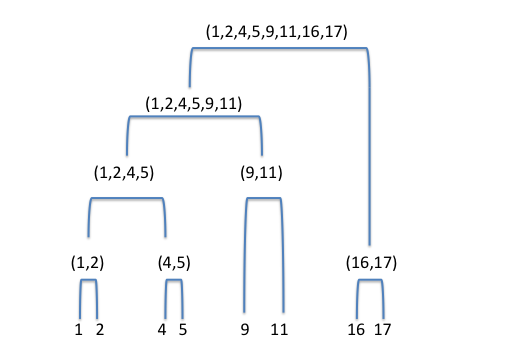
\includegraphics[scale=.5]{min_linkage.png}
\end{center}
b) \\
Step 1: \{1\} \{2\} \{4\} \{5\} \{9\} \{11\} \{16\} \{17\}\\
Step 2: \{1, 2\} \{4, 5\} \{9\} \{11\} \{16, 17\}\\
Step 3: \{1, 2\} \{4, 5\} \{9, 11\} \{16, 17\} \\
Step 4: \{1, 2, 4, 5\} \{9, 11\} \{16, 17\}\\
Step 5: \{1, 2, 4, 5\} \{9, 11, 16, 17\}\\
Step 6: \{1, 2, 4, 5, 9, 11, 16, 17\}
\begin{center}
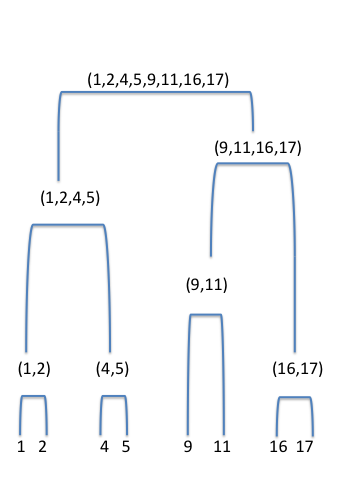
\includegraphics[scale=.5]{max_linkage.png}
\end{center}
\end{solution}

\newpage

\item{\bf Clustering Complexity}\\
\fbox{\parbox{\linewidth}{%
What is the ``big-O'' complexity of  HAC? 
What is the ``big-O'' complexity of K-means? 
Compare these.
%In terms of efficiency and determinism, when would HAC be a better method than divisive clustering?
}} \\
\begin{solution}
Let's look at what each algorithm does. For K-means, we have two steps, the assignment step and the centroid update. For the assignment step, we have $O(nKm)$, where $n$ is the size of data and $m$ is your dimensions because you have to compare each example with each of the centroids. Then, we have $O(nm)$ for the centroid update, since we will be calculating different averages for each of the centroids. Overall, with $T$ iterations we are left with $O(nKmT)$. 

For HAC, we start with each point in its own cluster, and combine the
two closest clusters until we are left with one big cluster. We get a
runtime of $O(n^2m)$ because we need to calculate the pairwise
distances for all $n$ examples.  In each of the $T_h$ clustering steps,
we then have $O(n^2)$ steps to use these pairwise distances and
whatever linkage we're using to compute the distances between existing
clusters.  Generally, $T_h$ is smaller than $m$ and the overall
complexity is $O(n^2m)$.

Comparing K-means and HAC, for large data sets we'd expect $KT$ in
K-means to be smaller than $n$, and thus K-means to be faster than
HAC.
\end{solution}

\vspace{3 in}

\item {\bf Scaling to large dimensions.}\\
\fbox{\parbox{\linewidth}{%
Explain the `curse of dimensionality' and how it is related to HAC.}}\\

\begin{solution}
The curse of dimensionality refers to the problem
% when volume exponentially increases with added dimensions. 
%
%
where distances become meaningless in very large dimensional spaces.
The problem is that the distance
between two examples with
some informative features but lots
and lots of random features 
will be approximately the same (try this out in simulation
if you don't see why!). 

This means that non-parametric (`instance based') 
methods such as HAC that use pairwise distances between
examples (vs between examples and prototypes in K-means) 
become less useful in higher dimensions.

%In the case of nonparametric methods like HAC, where distances are measured as a function of the dimensions, distances become less meaningful in higher dimensions. }}
\end{solution}

\if 0
\item {\bf Intuitively, when would top-down methods (e.g. divisive clustering) be a better method for clustering than bottom-up methods (e.g. HAC)? Give your answers in terms of data.}\\
\fbox{\parbox{\linewidth}{%
Bottom-up methods cluster based on local patterns without making decisions based on global patterns. Top-down clustering takes into account the global distribution. 
}}

\item {\bf K-Means++ }\\
\fbox{\parbox{\linewidth}{%
One way to initialize Lloyd's algorithm for K-Means is to randomly select some of the data to be the first cluster centers.  The easiest version of this would pick uniformly from among the data.  K-Means++ biases this distribution so that it is not uniform.  Explain in words how the distribution is non-uniform and why it should lead to better initializations.
}}
The K-Means++ algorithm iteratively adds cluster centers, drawing them from a distribution over the data.  This distribution is proportional to the squared distance of each datum from its nearest cluster center.  Thus K-Means++ tends to favor points that are distant from the existing centers and produce a more diverse set of centers.

\fi


\end{enumerate}


\end{document}
